\documentclass[11pt,a4paper,oneside]{article}
\usepackage[left=2cm,right=2cm,top=2cm,bottom=2cm]{geometry}
\usepackage[document]{ragged2e}
\usepackage[utf8]{inputenc}
\usepackage{amsmath}
\usepackage{amsfonts}
\usepackage{amssymb}
\usepackage{graphicx}
\usepackage{xcolor}
\usepackage{subfig}
\usepackage[output-decimal-marker={.}]{siunitx}
\usepackage{wrapfig}
\usepackage{lipsum}
\usepackage[toc]{appendix}
\usepackage{eso-pic}
\usepackage{hyperref}

\title{%
 \vspace{-2.0cm}
 Development of a procedure to Distinguish Residual Gas Annihilation from Annihilation on Trap Walls
}

\date{\vspace{-5ex}}
\author{Germano, Simone, Adriano}
\begin{document}

\AddToShipoutPicture*
    {\put(512.5,775){
\includegraphics[width = 0.125\textwidth]{../../logo/ALPHA_Logo.jpg}}}

\maketitle
\begin{abstract}
\centering
A fit procedure to separate the $\overline{H}$ annihilations on ALPHA trap walls from residual gas annihilations has been implemented and tested with a simple Monte Carlo toy model. The results and the procedure adopted to build up this model are presented in this note.
\end{abstract}


In the first part of this note we briefly discuss  the to identify a possible background source for ALPHA-2 and ALPHA-g experiments, which might be useful in the upcoming analyses of Lyman-$\alpha$ transition  and hyperfine splitting measurements. In the second part we will discuss the development of a Monte Carlo toy model to test the onset-finding algorithms of the hyperfine splitting measurement.
This study is done using \textit{ROOT} and \textit{RDataFrame}. All the software used for this analysis is can be found here: {\color{blue}{\url{https://github.com/Adrianodelvincio/ALPHA.git}}}

\section*{Annihilations Discrimination}

The ALPHA magnetic trap is designed to store the anti-hydrogen atoms that are produced during the mixing phase. The mixing phase consists on combining the anti-protons coming from ELENA with the positrons. 
The experiments in ALPHA hinge upon the detection of anti-hydrogen annihilation, to perform measurement pertaining to the asymmetries between matter and antimatter.\\
We take as a reference the hyperfine splitting of anti-hydrogen: the experiment consist on measuring the number of anti-hydrogen released from the magnetic trap subsequent to exposure to laser (microwave light) illumination with different frequencies. Most of the annihilations which are detected occur on the magnetic trap walls. Nevertheless, a certain percentage of this annihilation might arise from annihilation with residual gas. This second contribution is a potential source of background noise for the experiment. In light of this, we have devised a model to characterize and separate these two effects, that might potentially improve the results of the upcoming analyses.
\subsection*{Radius of the Annihilation Vertex}

Data about anti-hydrogen annihilation encompass several variables that are measured by the detectors. In order to distinguish the annihilation on the walls and that originating from residual gas, we have computed the radius (with respect to the center of the trap) $r$ of each annihilation vertex from the $X$ and $Y$ coordinates.
The radius distribution should to differ depending on the type of annihilation: for annihilation on the wall, the radius distribution should manifest a peak corresponding to the radius of the trap, while the events due to residual gas should mostly occur at smaller radius, near the geometric center of the trap.
To model the two contributions, we had different datasets available: 
\begin{itemize}
\item An almost pure annihilation on the walls dataset, taken during the $\SI{2}{\second}$ mixing phase of anti-protons and positions, to which we will refer as \textit{mixing} events.
\item An almost pure annihilation due to residual gas dataset, acquired during the exposure to laser illumination, but far away from the absorption peak (which we will indicate as \textit{UWlosses}).
\item An almost pure dataset of cosmic background events (supposed to be mainly muons) that are reconstructed erroneously as anti-hydrogen vertices. These data are taken when the magnetic trap does not contains the anti-hydrogen atoms.
\end{itemize}

The dataset are analysed separately, to build up different models for the radius distribution for each contribution. A list of run that are used in this analysis are reported in figure \href{fig:RunList}.

\subsection*{Annihilation on the walls}

The events contained in the \textit{mixing} dataset are supposed to be distributed around the radius of the magnetic trap, with a $\sigma$ given by different contribution, as for example the detector resolution in measuring the vertex coordinates. We have analysed only the events that pass the \textbf{cut 1} selection. The data are fitted assuming a gaussian model, see figure \ref{fig:MixingFit}.

\begin{figure}[hbtp]
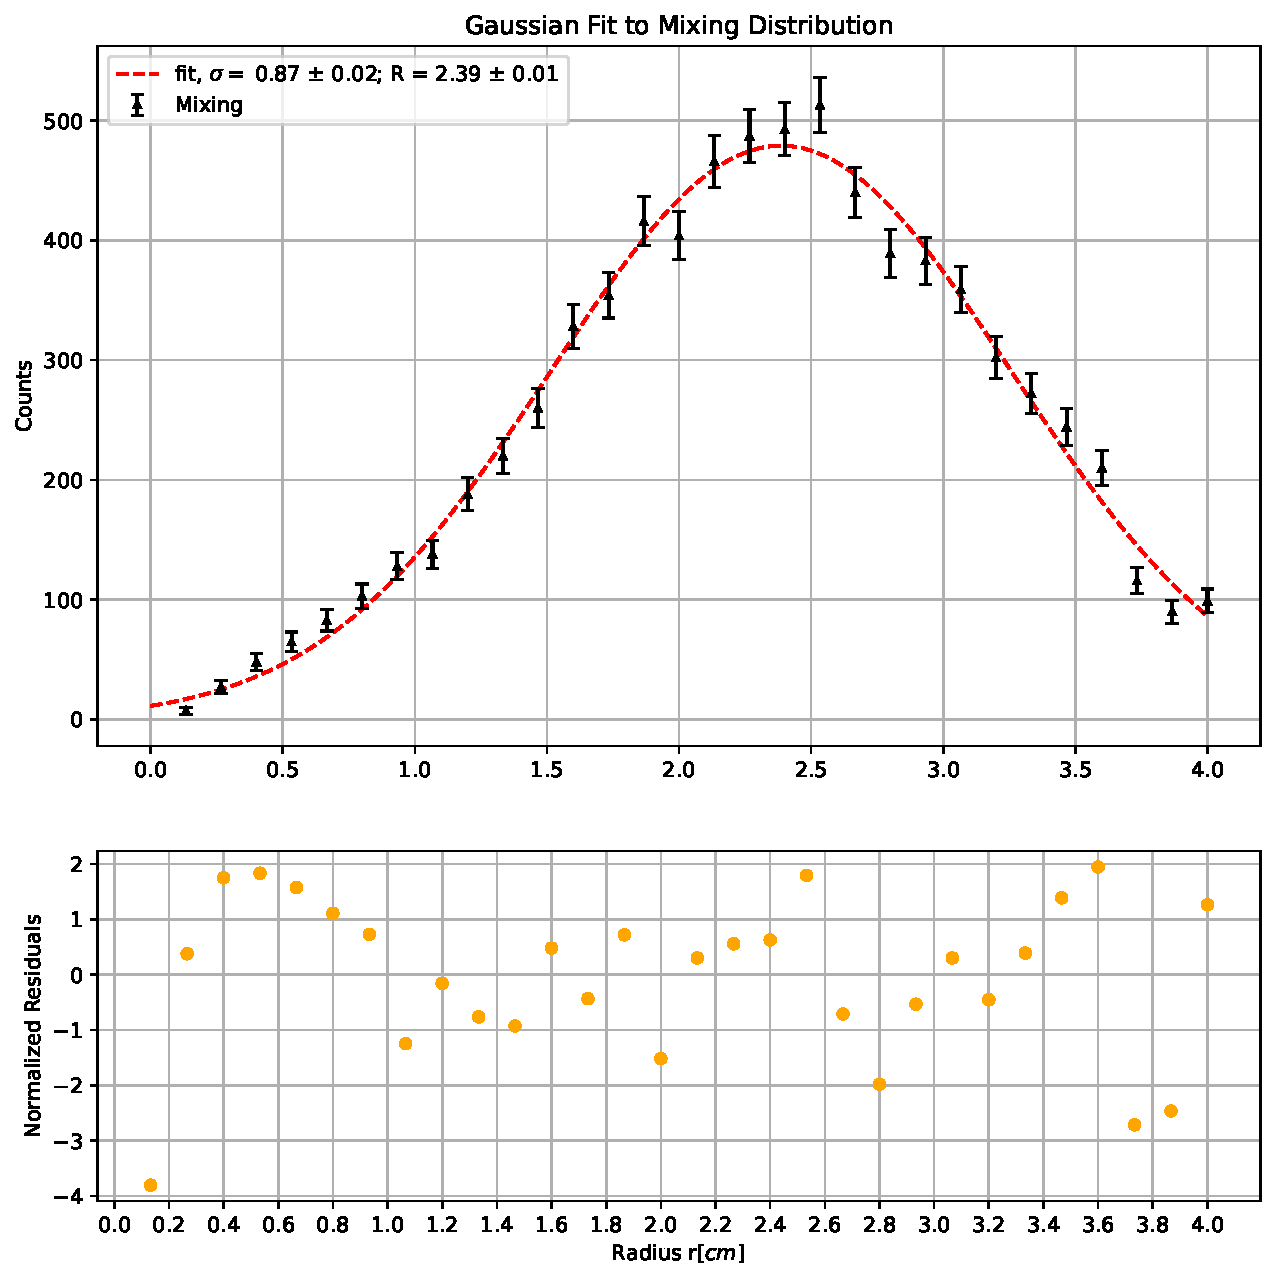
\includegraphics[width = 1\textwidth]{../PlotMLEfit/SingleModel/GaussianFitMixing.pdf}
\caption{Radius distribution of the annihilation vertices for the \textit{mixing} dataset. The red line is the gaussian model. On the bottom of the figure the residuals, assuming poissonian fluctuation ($\sigma = \sqrt{Counts}$).}
\label{fig:MixingFit}
\end{figure}

\subsection*{Annihilation due to Residual Gas}

For the Annihilation due to residual gas, we have used a different model compared to the one used before. We have assumed that the anti-hydrogen in the magnetic trap is roughly stored at the center, and that the $X$ and $Y$ coordinates of the annihilation vertices are normal distributed around the center of the magnetic trap. We assumed also that $\sigma_{x} = \sigma_{y}$, so there is no difference in $x,y$ directions. Under this assumptions, the radius distribution can be derived explicitly (\ref{sec:Rayleigh}), the analytic form is:

\begin{equation}
p(r) = \frac{r}{\sigma^{2}} \cdot  e^{ \dfrac{- r^{2}}{ 2 \sigma^{2}}}
\end{equation}

We have used this model to fit the \textit{UWlosses} data, considering only the events that pass the \textbf{cut 1} selection.
\begin{figure}[hbtp]

\centering
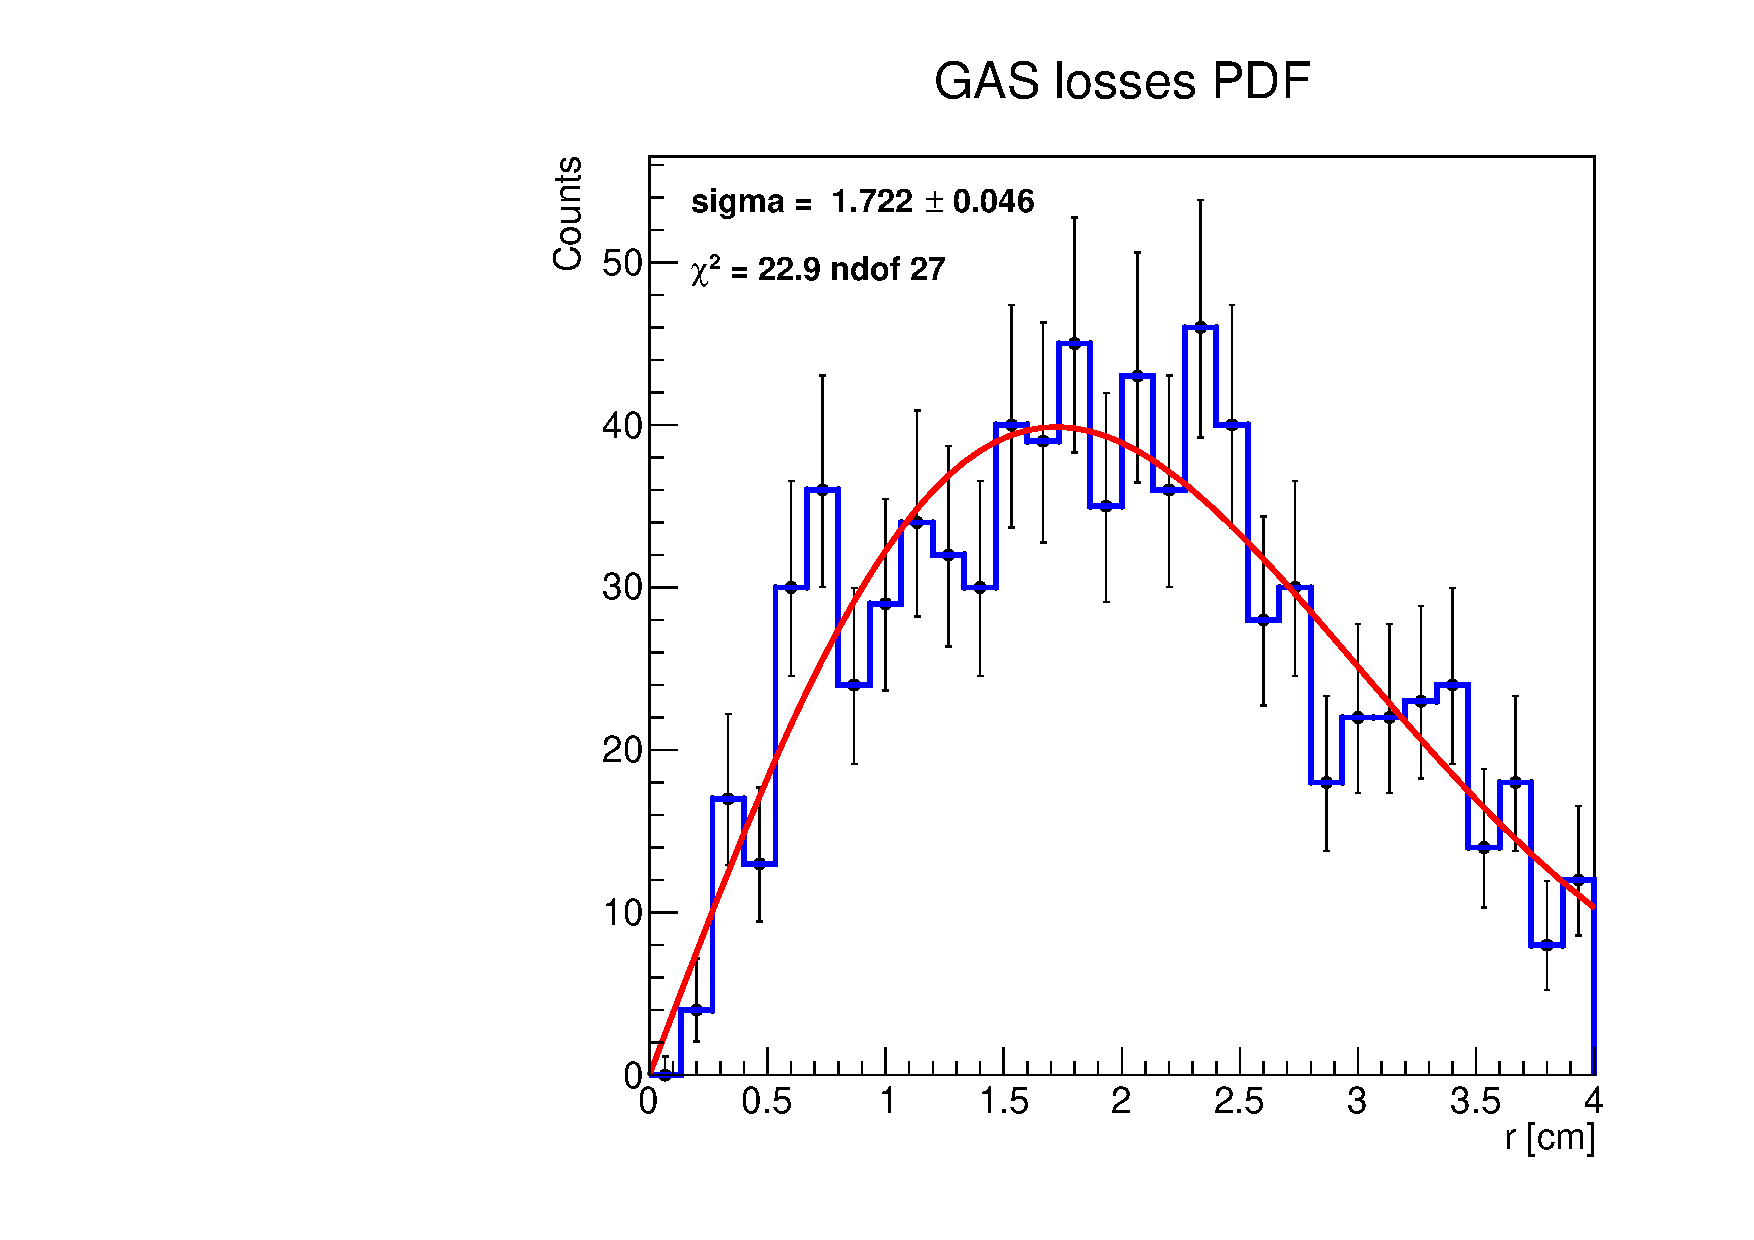
\includegraphics[width = 1\textwidth]{../PlotMLEfit/SingleModel/FitToUw.pdf}
\caption{ MLE fit of \textit{UWlosses} data. With SigRay we are indicating the $\sigma$ of the Rayleigh distribution.}
\end{figure}

\subsection*{Cosmic Background}

The cosmic background is expected to be uniform distributed in the trap volume. If the data are displayed in an histogram displaying the radius variable, then the quantity of events having a radius within the range $r$ and $r + dr$ will be directly proportional to the area $ 2 \pi r dr$ multiplied by the surface density of cosmic rays integrated during the time interval of data acquisition. It is reasonable to fit this distribution with a linear model:

\begin{figure}[hbtp]

\centering
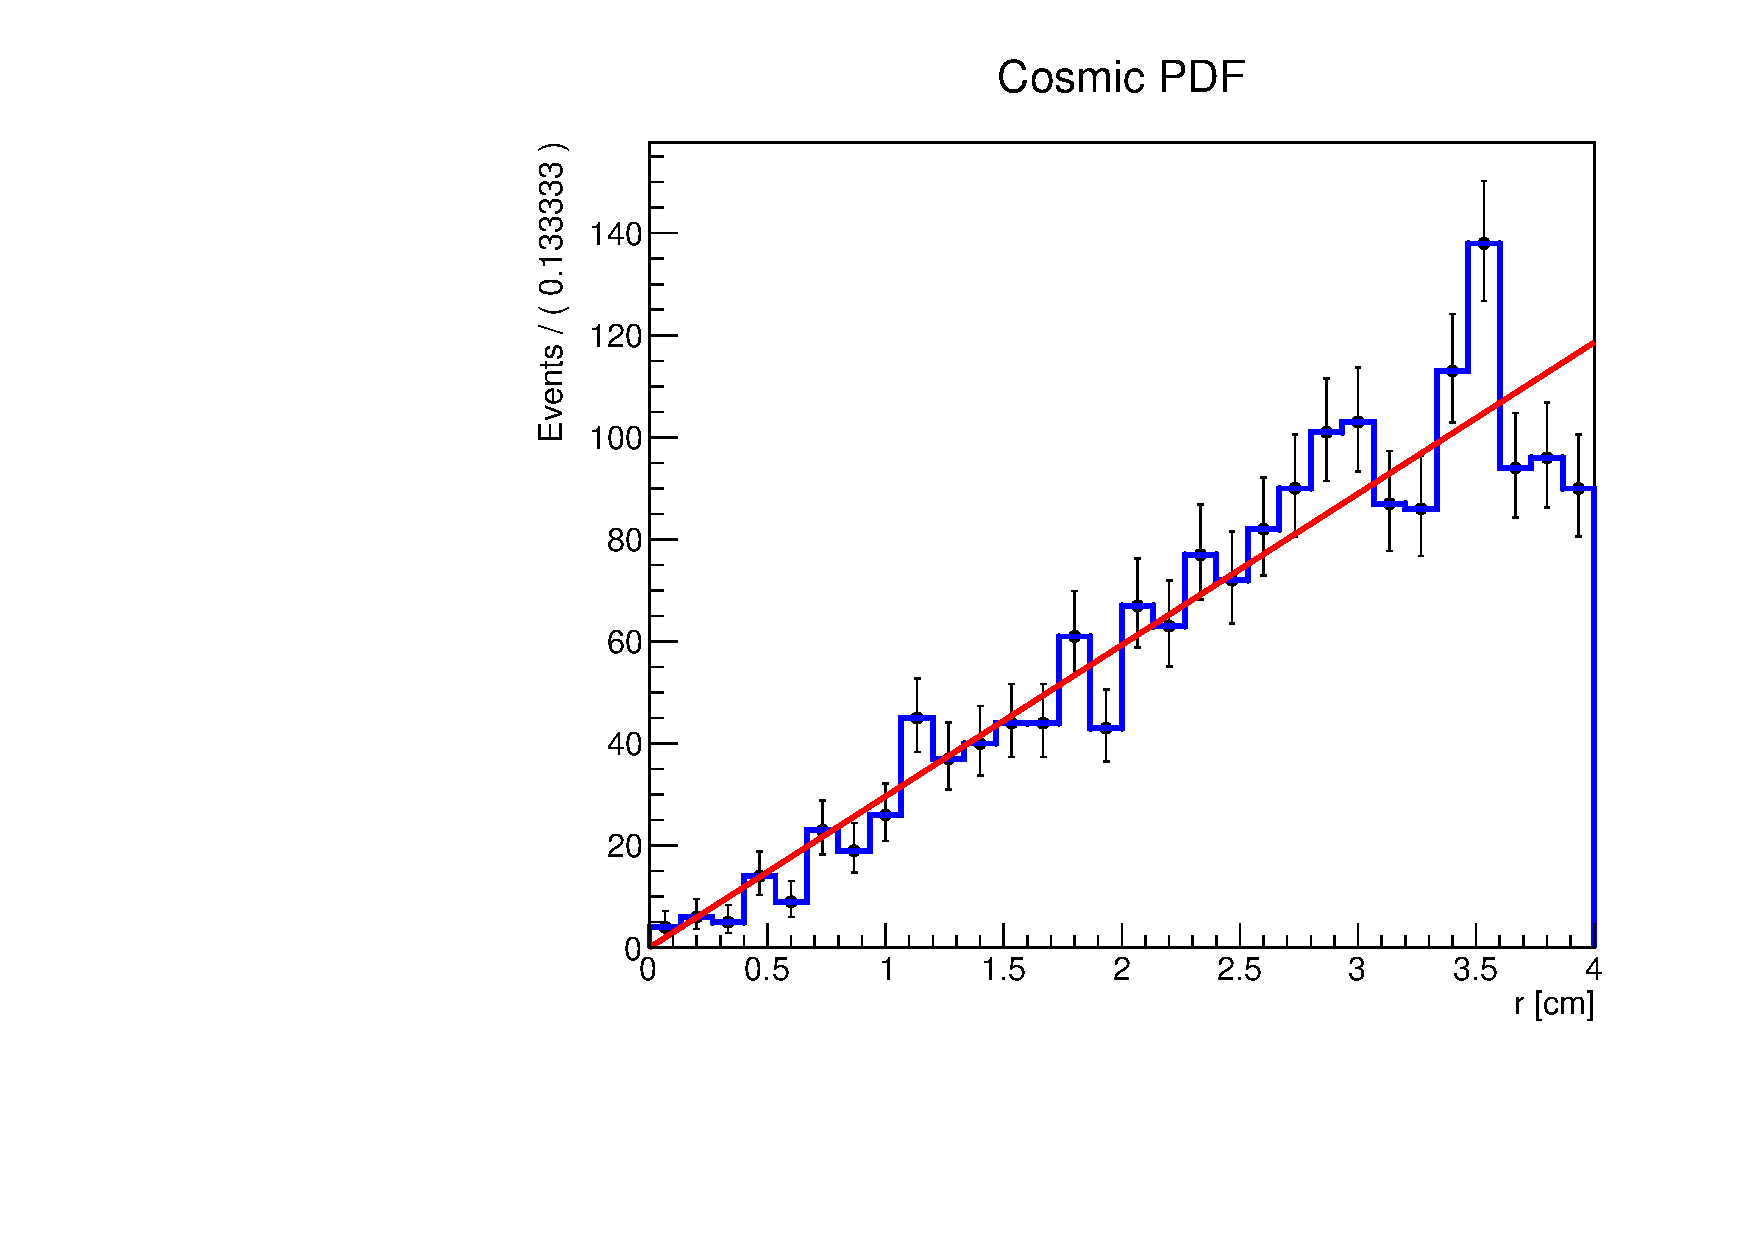
\includegraphics[width = 1\textwidth]{../PlotMLEfit/SingleModel/Cosmici_fit.pdf}
\caption{ MLE fit of the cosmic background dataset.}
\label{fig:CosmicBackground}
\end{figure}

From the amount of event show in figure \ref{fig:CosmicBackground}, we can determine the background rate. The data shown in this plot correspond to a time interval of $\SI{35000}{\second}$, and the amount of event is $1786$ which leads to:

\begin{equation} \label{eq:Rate}
rate = \frac{1786}{\SI{35000}{\second}} = \SI{0.051}{\second \tothe{-1}}
\end{equation}

\subsection{Normalized Pdfs}

The Normalized Pdfs are plotted together in figure \ref{fig:PdfsNormalized}
\begin{figure}[!hbtp]
\centering
\subfloat[][\emph{Normalized radius distributions.}\label{fig:PdfsNormalized}]{
	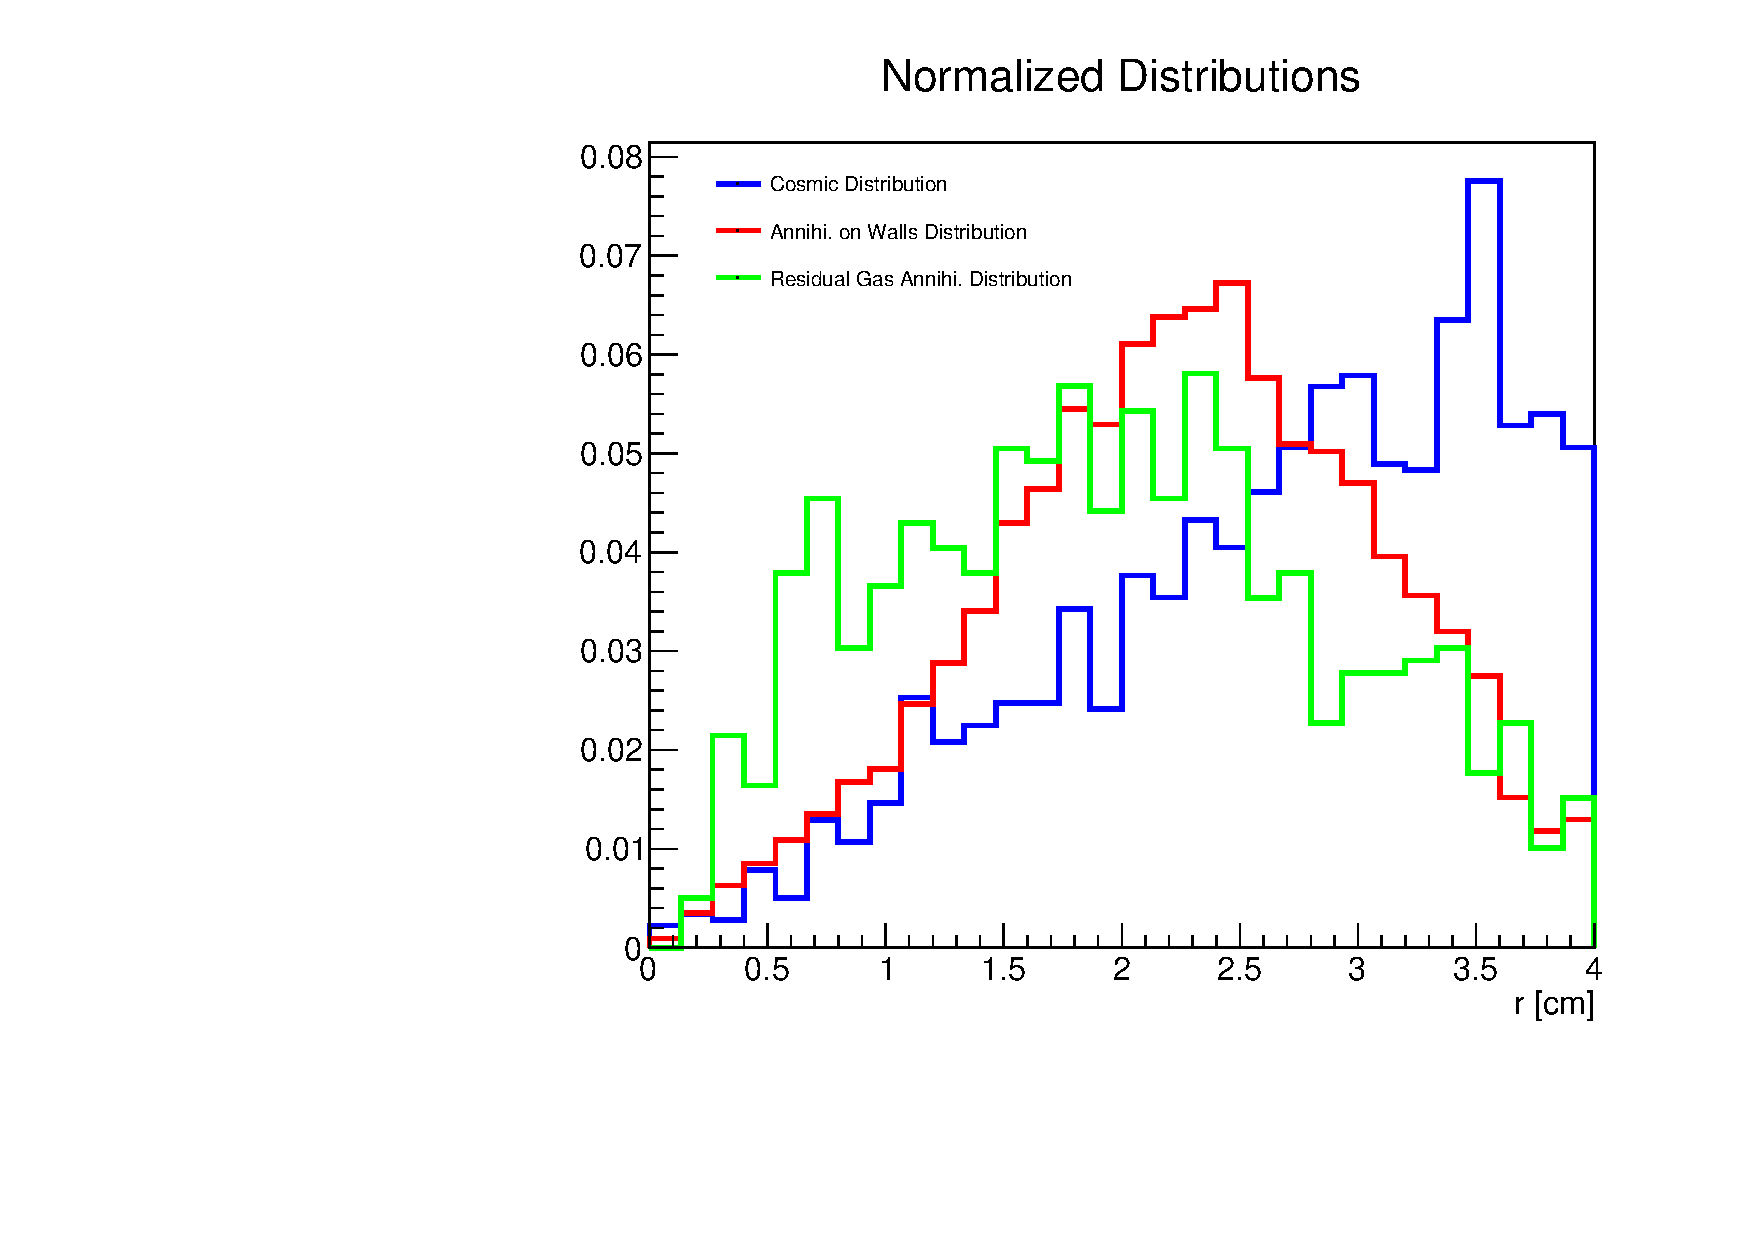
\includegraphics[width = .45\textwidth]{../PlotMLEfit/PdfTogether.pdf}}
\subfloat[][\emph{Radial density Pdfs.}\label{fig:RadialDensity}]{
	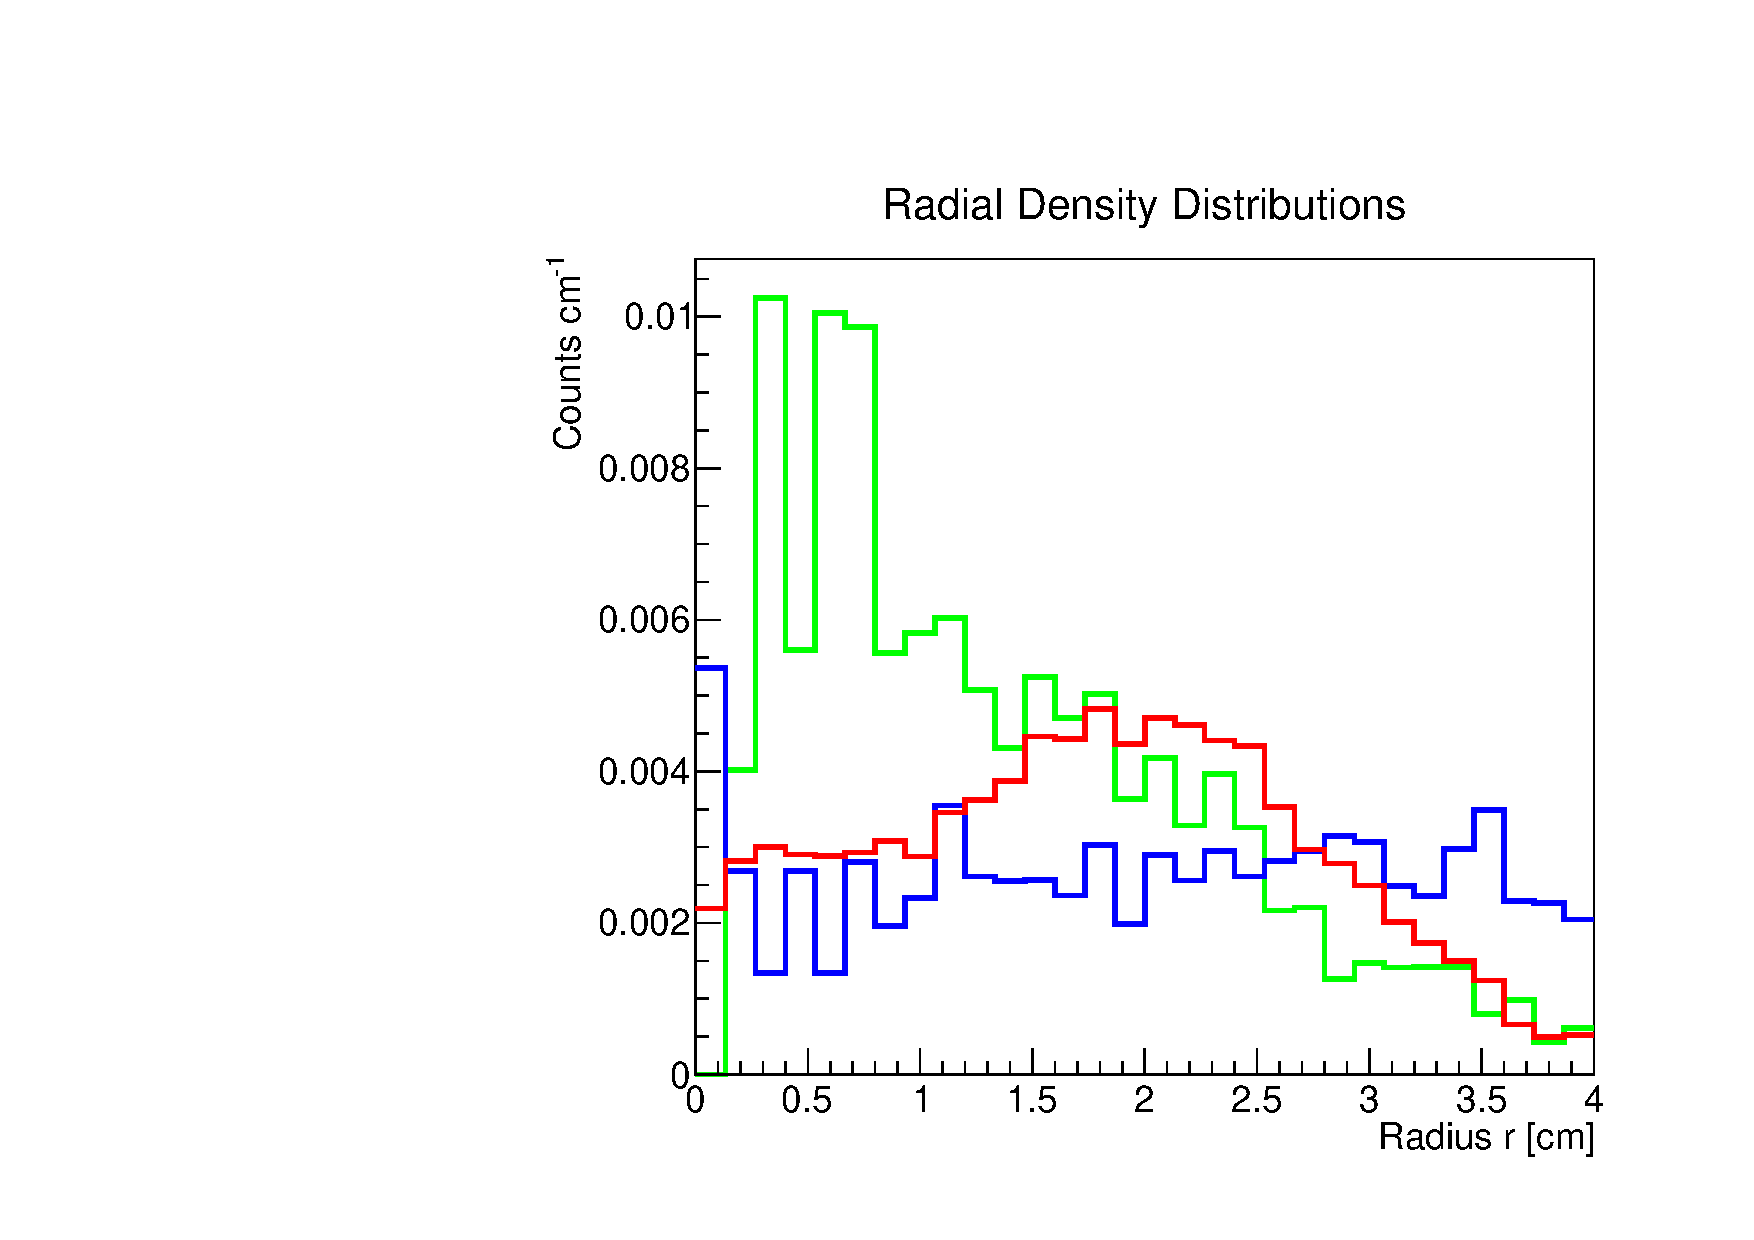
\includegraphics[width = .45\textwidth]{../PlotMLEfit/RadialDensity.pdf}}
\end{figure}

To correct for the different area corresponding to each bin, the values of each bin are divided by $ 2 \pi r$. The result are shown in figure :(\ref{fig:RadialDensity}). As we can see in this picture the annihilation due to residual gas shows a peak at $r \simeq 0$, while the annihilations on trap walls (that are indicated with the label \textit{mixing}) are distributed around $\simeq \SI{2}{ \centi \meter} - \SI{2.5}{\centi \meter}$. In the end the cosmic background seems to be uniform distributed in the range $\SI{0}{\centi \meter} - \SI{4}{\centi \meter}$.
\section*{Global Model}

After establishing individual models for each different process, we have constructed a comprehensive model made of three terms:

\begin{equation} \label{eq:GlobalModel}
\begin{split}
Model \quad = \quad &N_{wall} \cdot PDF_{wall} \\
	+ &N_{res \; gas} \cdot PDF_{res \; gas}\\ 
	+ &N_{cosmic} \cdot PDF_{cosmic}
\end{split} 
\end{equation} 

where $N_{wall}$, $N_ {res \; gas}$ and $N_{cosmic}$ are the number of annihilation on traps walls, due to residual gas and cosmic events, respectively.
The free parameters of this global model are only $N_{wall}$ and $N_{res \; gas}$. When using this model, $N_{cosmic}$ is a constant parameter, adjusted to the expected number of cosmic events of the particular run which is analysed.
We have tested this model with an ad-hoc Monte Carlo simulation. The objective of the simulation is to asses whether a maximum likelihood fit with the model in equation \ref{eq:GlobalModel} is able to recover the values of $N_{wall}$ and $N_{res \; gas}$ from the simulated data, and also determine the accuracy of this method. 
We have generated data following the model in eq. \ref{eq:GlobalModel}, with the total number of events sampled by a poisson distribution with mean $N_{tot \, exp} = 1000$ (to account for the statistical fluctuation in the number of event). The expected number of annihilations on walls and residual gas is $N_{wall} , N_{res \, gas} = (500,500)$ . The expected value of $N_{cosmic}$ is fixed to $10.2$ events. \footnote{ This value is chosen as the expected number of cosmic events for the run ...}.
The data are fitted with the same model used for the generation, with the only free parameters $N_{wall} , N_{res \, gas}$. This procedure is repeated for $N_{trial} = 1000$ times. For each individual trial we compute the quantity:
\begin{equation} \label{eq:ParmasReco}
\dfrac{N_{fit} - N_{gen}}{\sigma}
\end{equation}

That is the difference between the expected number of event used in the generation and the value retrieved from the fit, weighted with the error on the parameter given by the fit.  These quantities are shown in figure \ref{fig:ReconstructedParameters}

\begin{figure}[hbtp]
\centering
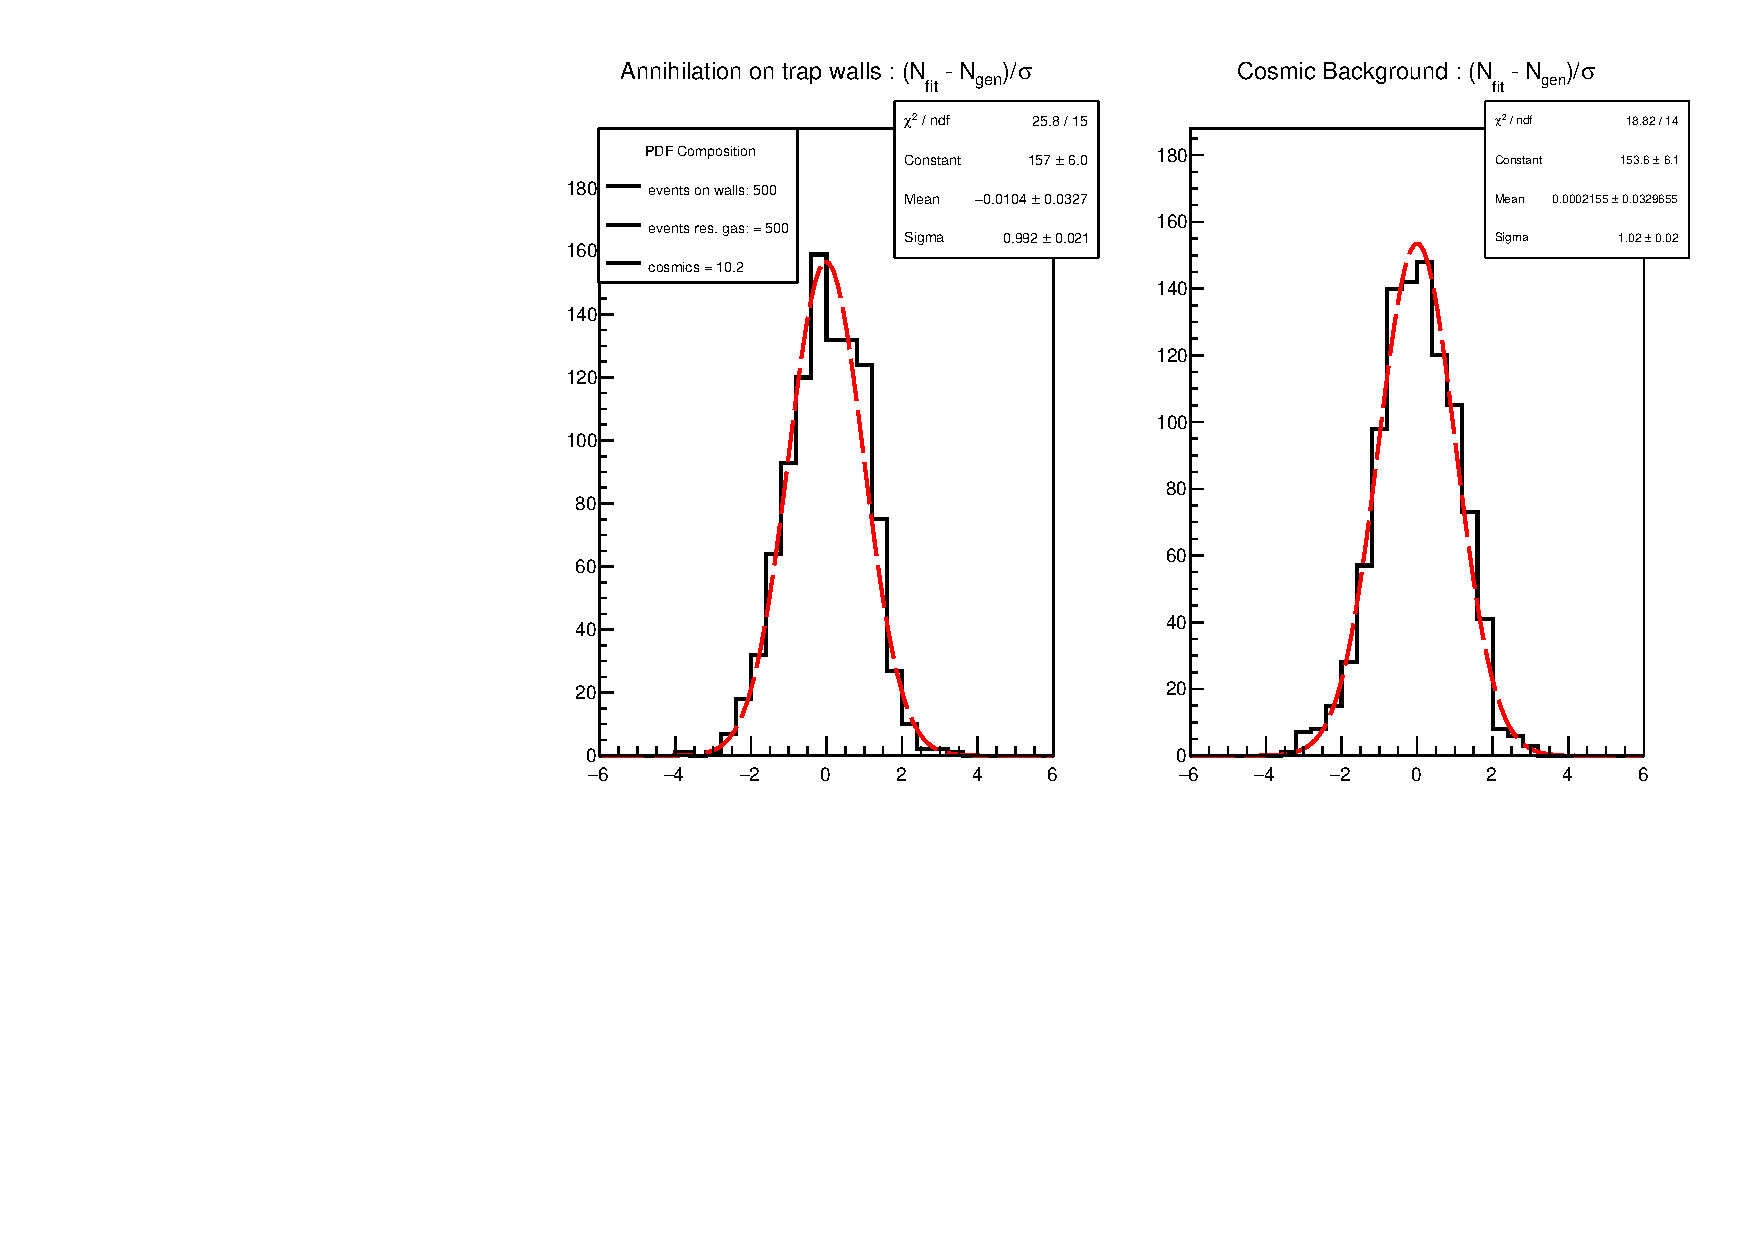
\includegraphics[width = \textwidth]{../PlotMLEfit/N1000/Reconstruced_(500,500).pdf}
\caption{Weighted difference between the reconstructed parameters and the values used in the data generation as defined in equation \ref{eq:ParmasReco}.}
\label{fig:ReconstructedParameters}
\end{figure}



\appendix
\section{Derivation of the Rayleigh Distribution}
\label{sec:Rayleigh}

The Rayleigh distribution arises when the radius of two independent normal variables $x,x$ is considered.

\begin{equation*}
r = \sqrt{x^{2} + y^{2}}
\end{equation*} 


In principle it is possible to compute directly the radius distribution from the change of variable, however there is a straightforward demonstration. If we consider the cumulative $F_{r}$, we can write that:

\begin{equation*}
F_{r}(r, \sigma) = \int \int_{ \sqrt{x^{2} + y^{2}} < r} N_{x}(\sigma) N_{y}(\sigma) \, dx dy
\end{equation*}

Where $N_{x}$ and $N_{y}$ are the normal distributions. Switching from Cartesian to polar coordinates, the cumulative is:

\begin{equation*}
F_{r}(r, \sigma) =  \int_{0}^{2 \pi} \int_{0}^{r} \frac{1}{2 \pi \sigma^{2}}  e^{ \frac{- r^{2}}{2 \sigma^{2}}} \; r  dr d\theta
\end{equation*}


The \textit{pdf} is given by the derivative of the cumulative function, and we end with the Rayleigh distribution:


\begin{equation}
p(r) = \frac{r}{\sigma^{2}} \cdot  e^{ \dfrac{- r^{2}}{ 2 \sigma^{2}}}
\end{equation}


\section{Run List}
\label{fig:RunList}

\begin{figure}[hbtp]
\centering
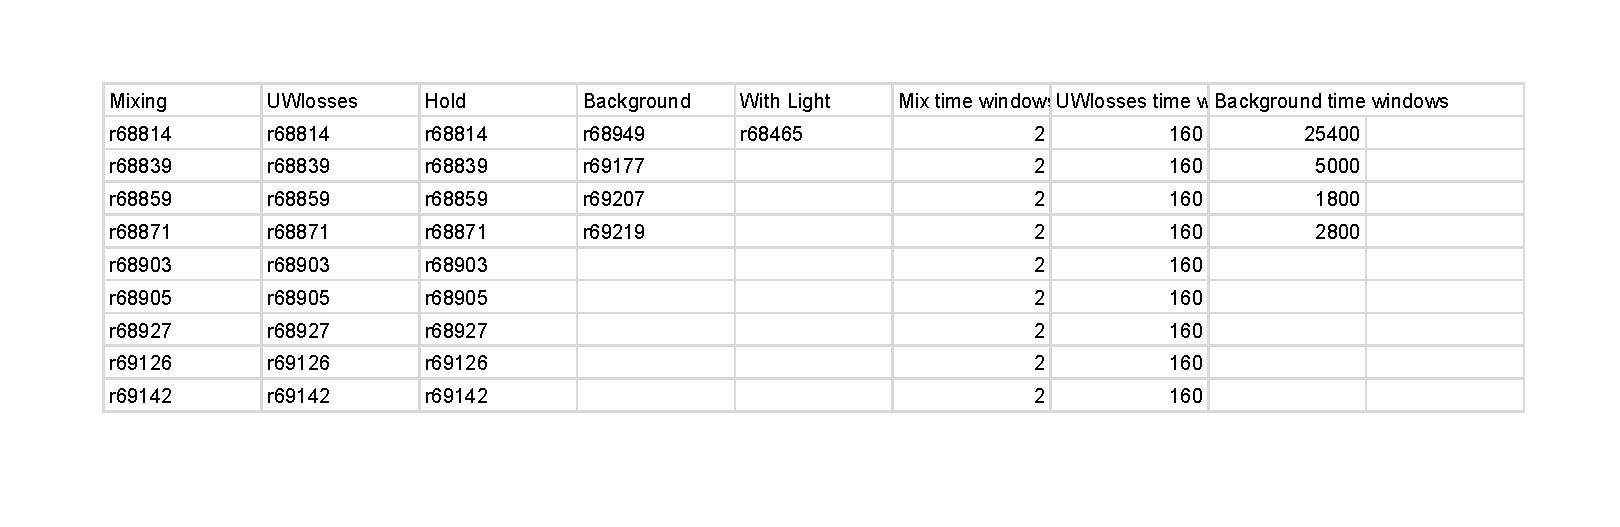
\includegraphics[width = 1\textwidth]{../PlotMLEfit/ListofRun-cropped.pdf}
\caption{List of runs analysed.}
\end{figure}

\end{document}